%% ============================================================
%% EJ-228 Cylinder — Vikuiti vs TIR-only light yield study
%% Geant4 11.4 simulation | rrios / dowiyogo@gmail.com
%% ============================================================
\documentclass[aspectratio=169,10pt]{beamer}

\usetheme{Boadilla}
\usecolortheme{seahorse}
\useinnertheme{circles}
\setbeamertemplate{navigation symbols}{}
\setbeamertemplate{footline}[frame number]

\usepackage[utf8]{inputenc}
\usepackage[T1]{fontenc}
\usepackage{lmodern}
\usepackage{booktabs}
\usepackage{siunitx}
\usepackage{xcolor}
\usepackage{graphicx}
\usepackage{tikz}
\usetikzlibrary{shapes.geometric,arrows.meta,decorations.pathmorphing,patterns,calc}

% ── Colors ───────────────────────────────────────────────────────────────────
\definecolor{vikuiti}{RGB}{30,80,180}    % blue: Vikuiti
\definecolor{tironly}{RGB}{200,100,10}   % orange: TIR-only
\definecolor{scintgr}{RGB}{60,160,60}    % scintillator green
\definecolor{airgap}{RGB}{200,230,255}   % light blue: air
\definecolor{sipmcol}{RGB}{30,30,180}    % SiPM blue
\definecolor{mylarGr}{RGB}{180,180,180}  % Vikuiti grey

% ── Title ────────────────────────────────────────────────────────────────────
\title[EJ-228 Cylinder — Vikuiti vs TIR]%
      {Light Yield Study: Vikuiti~3M~ESR vs TIR-only\\
       on an EJ-228 Plastic Scintillator Cylinder}

\subtitle{Geant4 11.4 MT Simulation --- feat/ej228-cylinder \&
          feat/ej228-tir-only}

\author{R.~Rios}
\institute{Simulated using \texttt{ej204} framework}
\date{\today}

% ─────────────────────────────────────────────────────────────────────────────
\begin{document}

\begin{frame}
  \titlepage
\end{frame}

% ─────────────────────────────────────────────────────────────────────────────
\section{Detector Geometry}

\begin{frame}{Detector Geometry — EJ-228 Cylinder}

\begin{columns}[T]
  %% ── Left: TikZ cross-section ──────────────────────────────────────────────
  \begin{column}{0.52\textwidth}
  \centering
  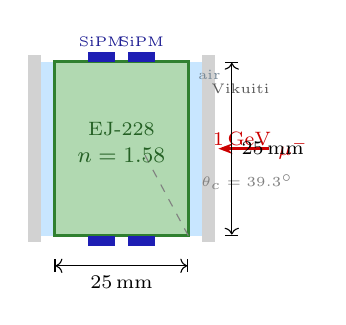
\begin{tikzpicture}[scale=0.85,every node/.style={font=\scriptsize}]

    % Vikuiti mantle (full height annulus)
    \fill[mylarGr!60] (-1.4,-1.4) rectangle (-1.2,1.4);
    \fill[mylarGr!60] ( 1.2,-1.4) rectangle ( 1.4,1.4);

    % Air gap
    \fill[airgap] (-1.2,-1.3) rectangle (-1.0,1.3);
    \fill[airgap] ( 1.0,-1.3) rectangle ( 1.2,1.3);

    % Scintillator body
    \fill[scintgr!40] (-1.0,-1.3) rectangle (1.0,1.3);
    \draw[scintgr!80!black,very thick] (-1.0,-1.3) rectangle (1.0,1.3);

    % SiPMs top (4 in 2x2 grid shown as 2 rectangles in side view)
    \fill[sipmcol] (-0.5, 1.3) rectangle (-0.1, 1.45);
    \fill[sipmcol] ( 0.1, 1.3) rectangle ( 0.5, 1.45);
    \fill[sipmcol] (-0.5,-1.45) rectangle (-0.1,-1.3);
    \fill[sipmcol] ( 0.1,-1.45) rectangle ( 0.5,-1.3);

    % Muon arrow (entering from right through mantle)
    \draw[red!80!black,very thick,-{Stealth[length=5pt]}]
      (2.2,0) -- (1.45,0);
    \node[red!80!black,right] at (2.2,0) {$\mu^-$};
    \node[red!80!black] at (1.8,0.15) {\scriptsize 1\,GeV};

    % Dashed TIR critical angle
    \draw[dashed,gray] (1.0,-1.3) -- (0.3,0.0);
    \node[gray,right,align=left] at (1.05,-0.5)
      {\tiny $\theta_c=39.3^\circ$};

    % Labels
    \node[scintgr!60!black] at (0, 0.3) {EJ-228};
    \node[scintgr!60!black] at (0,-0.1) {\footnotesize $n=1.58$};
    \node[airgap!60!black,right] at (1.0, 1.1) {\tiny air};
    \node[mylarGr!50!black,right] at (1.2, 0.9) {\tiny Vikuiti};
    \node[sipmcol!80!black] at (-0.3, 1.6) {\tiny SiPM};
    \node[sipmcol!80!black] at ( 0.3, 1.6) {\tiny SiPM};

    % Dimension annotation
    \draw[|<->|,thin] (-1.0,-1.75) -- (1.0,-1.75)
      node[midway,below] {\SI{25}{mm}};
    \draw[|<->|,thin] (1.65,-1.3) -- (1.65,1.3)
      node[midway,right] {\SI{25}{mm}};

  \end{tikzpicture}

  \vspace{0.3em}
  {\footnotesize Side cross-section (XZ plane)}
  \end{column}

  %% ── Right: parameter table ────────────────────────────────────────────────
  \begin{column}{0.46\textwidth}
  \small
  \begin{block}{Geometry}
    \begin{tabular}{@{}ll@{}}
      Scintillator & EJ-228 (PVT-based) \\
      Shape        & Cylinder \\
      Diameter     & \SI{25}{mm} \\
      Height       & \SI{25}{mm} \\
      Refractive index & $n = 1.58$ \\
      Decay time   & \SI{1.4}{ns} \\
      Light yield  & \SI{9700}{ph/MeV} \\
      Attenuation  & \SI{110}{cm} \\
    \end{tabular}
  \end{block}

  \begin{block}{Surfaces}
    \begin{tabular}{@{}ll@{}}
      Mantle (scint/air) & Polished + TIR \\
      $\theta_c$ & $\arcsin(1/1.58)=39.3^\circ$ \\
      Vikuiti wrap & R = 0.98, specular \\
      Air gap & \SI{0.1}{mm} \\
      Cap faces & Polished, free \\
    \end{tabular}
  \end{block}

  \begin{block}{Readout}
    \begin{tabular}{@{}ll@{}}
      SiPMs & AFBR-S4N66P024M \\
      Layout & $2\times2$ per cap \\
      Total & 8 SiPMs (4 top + 4 bot) \\
      Active area & $6\times6\,\si{mm^2}$ each \\
      Coupling & polished, $n=1.58$ \\
    \end{tabular}
  \end{block}
  \end{column}
\end{columns}

\end{frame}

% ─────────────────────────────────────────────────────────────────────────────
\begin{frame}{Two Configurations Compared}

\begin{columns}[T]

  \begin{column}{0.48\textwidth}
  \begin{alertblock}{\textcolor{vikuiti}{\textbf{Config A — Vikuiti 3M ESR}}}
    \begin{itemize}
      \item Annular Vikuiti wrap on mantle
      \item \SI{0.1}{mm} air gap + \SI{0.1}{mm} Vikuiti shell
      \item Specular reflectance $R = 0.98$
      \item Photons escaping TIR reflected back
      \item Dielectric-metal surface model (Unified)
    \end{itemize}
    \vspace{0.3em}
    \textbf{Branch:} \texttt{feat/ej228-cylinder}
  \end{alertblock}
  \end{column}

  \begin{column}{0.48\textwidth}
  \begin{alertblock}{\textcolor{tironly}{\textbf{Config B — TIR-only (bare air)}}}
    \begin{itemize}
      \item No reflective wrap on mantle
      \item \SI{0.1}{mm} air gap present
      \item Photons escaping TIR are \textbf{lost}
      \item Only TIR photons ($\theta > 39.3^\circ$) survive
      \item Caps remain open in both configs
    \end{itemize}
    \vspace{0.3em}
    \textbf{Branch:} \texttt{feat/ej228-tir-only}
  \end{alertblock}
  \end{column}

\end{columns}

\vspace{0.8em}

\begin{block}{Simulation Parameters (identical for both)}
  \centering
  \begin{tabular}{@{}llll@{}}
    \toprule
    Particle & Energy & Statistics & Generator position \\
    \midrule
    $\mu^-$ (horizontal) & \SI{1}{GeV} & 5000 events & $(+80, 0, 0)\,\si{mm}$ \\
    \bottomrule
  \end{tabular}
\end{block}

\vspace{0.3em}
{\footnotesize GROUPVEL aliasing fix applied (world air gets $v_g = c/1.58$). Finite scintillation rise time enabled.}

\end{frame}

% ─────────────────────────────────────────────────────────────────────────────
\section{Simulation Results}

\begin{frame}{Total $N_\text{pe}$ per Event}

\begin{columns}[c]
  \begin{column}{0.60\textwidth}
    \centering
    \includegraphics[width=\linewidth]{npe_total_comparison.png}
  \end{column}
  \begin{column}{0.38\textwidth}
    \begin{block}{\footnotesize How this plot is produced}
    \footnotesize
    For each of the 5\,000 simulated events, all photon hits in any of the
    8 SiPMs are counted ($N_\text{pe}$ per event) and filled into two overlaid
    histograms.  Dashed vertical lines mark the means.\\[0.4em]
    The Landau-like shape arises from stochastic energy deposition of a MIP
    (Bethe--Bloch + $\delta$-rays) along the \SI{25}{mm} scintillator track.
    \end{block}
  \end{column}
\end{columns}

\end{frame}

% ─────────────────────────────────────────────────────────────────────────────
\begin{frame}{$N_\text{pe}$ per Cap — Top and Bottom}

  \begin{center}
    \includegraphics[width=0.92\textwidth]{npe_percap_comparison.png}
  \end{center}

  \vspace{-0.5em}
  {\footnotesize
  Top cap (IDs 0--3) and bottom cap (IDs 4--7) show nearly identical counts,
  confirming the expected Z-symmetry of the muon track through the cylinder centre.
  }

\end{frame}

% ─────────────────────────────────────────────────────────────────────────────
\begin{frame}{$N_\text{pe}$ per Individual SiPM (log scale)}

  \begin{center}
    \includegraphics[width=0.72\textwidth]{npe_persipm_comparison.png}
  \end{center}

  \vspace{-0.3em}
  {\footnotesize
  \textbf{Bar chart}: each bar = mean $N_\text{pe}$ per event for that single SiPM
  (left bar = Vikuiti, right bar = TIR-only; log $y$-scale so the 2.34$\times$ ratio is directly visible).
  IDs~0,1,4,5 ($x=\SI{-3}{mm}$) collect $\sim\!2\%$ more than IDs~2,3,6,7 ($x=\SI{+3}{mm}$):
  consistent with the muon entering from the $+x$ mantle side.
  }

\end{frame}

% ─────────────────────────────────────────────────────────────────────────────
\begin{frame}{Numerical Comparison}

\begin{center}
\renewcommand{\arraystretch}{1.3}
\begin{tabular}{@{}lSSS@{}}
  \toprule
  \textbf{Observable} &
  {\textbf{Vikuiti $R=0.98$}} &
  {\textbf{TIR-only}} &
  {\textbf{Ratio}} \\
  \midrule
  Total photon hits         & 48313553 & 20642555 & 2.340 \\
  $\langle N_\text{pe}\rangle$ /event  & 9662.7 & 4128.5 & 2.340 \\
  $\sigma_{N_\text{pe}}$ /event        & 2237.9 & 937.3  &  {---} \\
  Median $N_\text{pe}$ /event          & 8969   & 3840   & 2.335 \\
  $\langle N_\text{pe}\rangle$ top cap & 4831.7 & 2063.1 & 2.342 \\
  $\langle N_\text{pe}\rangle$ bot cap & 4831.0 & 2065.4 & 2.339 \\
  Detection efficiency (\%) & 20.26 & 8.66 & 2.340 \\
  Photons killed in world   & 148070008 & 205994125 & 0.719 \\
  \bottomrule
\end{tabular}
\end{center}

\vspace{0.4em}
\begin{alertblock}{}
  \centering
  Vikuiti 3M ESR increases light collection by a factor of
  \textbf{\textcolor{vikuiti}{$2.34\times$}} compared to TIR-only confinement.
\end{alertblock}

\end{frame}

% ─────────────────────────────────────────────────────────────────────────────
\section{Timing Resolution}

\begin{frame}{Timing Resolution Setup}

\begin{columns}[T]
  \begin{column}{0.56\textwidth}
  \begin{block}{Method — $k$-th photon order statistics}
    \begin{enumerate}\setlength\itemsep{0.25em}
      \item Per event: sort all photon arrival times on the \textbf{top cap}
            (4 SiPMs combined).
      \item Extract $t_{(k)}$ = $k$-th earliest arrival time.
      \item Build histogram of $t_{(k)}$ across all 5000 events.
      \item Fit Gaussian to the \textbf{core} ($\pm2\sigma_{68\%}$ range) —
            robust against the right-skew intrinsic to order statistics.
      \item $\sigma(k)$ = width of Gaussian fit = timing resolution
            when triggering on the $k$-th photon.
    \end{enumerate}
  \end{block}

  \vspace{0.4em}
  \begin{block}{Expectation}
  \small
  \begin{tabular}{@{}l@{$\;\Rightarrow\;$}l@{}}
    $k=1$       & fastest direct-path photon; $\sigma$ set by geometry \\
    $k\uparrow$ & photon mix shifts; $\sigma(k)$ non-trivial \\
    Vikuiti     & $2.34\times$ more photons $\to$ advantage at large $k$ \\
  \end{tabular}
  \end{block}
  \end{column}

  \begin{column}{0.42\textwidth}
  \begin{block}{Photon count per event (top cap)}
    \renewcommand{\arraystretch}{1.2}
    \begin{tabular}{@{}lS[table-format=4.0]@{}}
      \toprule
      Config & {$\langle N_\text{pe}\rangle$ top cap} \\
      \midrule
      Vikuiti R=0.98 & 4832 \\
      TIR-only       & 2063 \\
      \midrule
      Ratio & 2.34 \\
      \bottomrule
    \end{tabular}

    \vspace{0.6em}
    {\footnotesize
    Even at $k=50$, TIR-only uses rank $50/2063 = 2.4\%$\\
    while Vikuiti uses rank $50/4832 = 1.0\%$ — earlier\\
    photons with smaller geometric spread.
    }
  \end{block}
  \end{column}
\end{columns}

\end{frame}

% ─────────────────────────────────────────────────────────────────────────────
\begin{frame}{$\sigma(k)$ vs $k$ — Timing Resolution Curves}

  \begin{center}
    \includegraphics[width=0.62\textwidth]{timing_sigma_vs_k.png}
  \end{center}

  \vspace{-0.5em}
  {\footnotesize
  Filled markers: $\sigma_\text{Gauss}$ (Gaussian fit on $\pm2\sigma_{68\%}$ core).
  Dashed lines: $\sigma_\text{IQR}=\text{IQR}/1.349$ (robust; both agree).
  Arrows mark the \textbf{optimal threshold} $k_\text{opt}\approx8$ (same for both configs),
  where $\sigma_\text{opt}\approx\SI{6.7}{ps}$.
  Non-monotonic shape: dip at $k\approx8$ = direct-path regime;
  rise at $k\approx20$ = onset of once-reflected photons with larger path spread.
  }

\end{frame}

% ─────────────────────────────────────────────────────────────────────────────
\begin{frame}{$t_{(k)}$ Distributions — Gaussian Fits (top cap)}

  \begin{center}
    \includegraphics[width=0.72\textwidth]{timing_fits_panels.png}
  \end{center}

  \vspace{-0.3em}
  {\footnotesize
  Each panel: $\Delta t_k = t_{(k)} - \mathrm{median}(t_{(k)})$ across 5000 events.
  Curves: Gaussian fits on the $\pm2\sigma_{68\%}$ core (solid = Vikuiti, dashed = TIR-only).
  Near $k_\text{opt}\approx8$, distributions are narrow and near-Gaussian (k=5, 10 panels).
  Vikuiti advantage clear only at $k=50$: $\sigma_V=\SI{7.3}{ps}$ vs $\sigma_T=\SI{10.2}{ps}$.
  }

\end{frame}

% ─────────────────────────────────────────────────────────────────────────────
\begin{frame}{Timing Resolution — Numerical Summary}

\begin{center}
\small
\renewcommand{\arraystretch}{1.25}
\begin{tabular}{@{}lSSSS@{}}
  \toprule
  \textbf{$k$} &
  {\textbf{$\sigma_V$ [ps]}} &
  {\textbf{$\sigma_T$ [ps]}} &
  {\textbf{$\sigma_V/\sigma_T$}} &
  {\textbf{Notes}} \\
  \midrule
  1              & 10.4 & 10.5 & 0.987 & {geometric floor} \\
  2              &  8.4 &  8.4 & 0.999 & {direct paths} \\
  5              &  6.9 &  6.8 & 1.017 & {near optimum} \\
  \bfseries{8 ($k_\text{opt}$)} & \bfseries{6.7} & \bfseries{6.6} & \bfseries{1.02} & \bfseries{optimal threshold} \\
  10             &  6.8 &  6.9 & 0.993 & {direct paths} \\
  20             & 10.0 & 10.3 & 0.968 & {reflected onset} \\
  50             &  7.3 & 10.2 & \textbf{0.718} & {Vikuiti 28\% better} \\
  \bottomrule
\end{tabular}
\end{center}

\vspace{0.4em}
\begin{columns}[T]
  \begin{column}{0.48\textwidth}
  \begin{alertblock}{Key result}
    $\sigma \sim 7$--$11\,\si{ps}$ in the ideal (no electronics jitter) limit.
    This reflects geometric spread in photon path lengths
    ($\sim\!\SI{1.5}{mm}$ path-length variation at $v=c/1.58$).
  \end{alertblock}
  \end{column}
  \begin{column}{0.48\textwidth}
  \begin{alertblock}{Vikuiti advantage}
    Negligible for $k \leq 20$.
    At $k=50$: Vikuiti gives \textbf{28\% better} timing
    ($\sigma_V / \sigma_T = 0.72$) because higher $N_\text{pe}$ keeps
    the 50th photon at an earlier rank in the time distribution.
  \end{alertblock}
  \end{column}
\end{columns}

\end{frame}

% ─────────────────────────────────────────────────────────────────────────────
\section{Physics Interpretation}

\begin{frame}{Physics Interpretation}

\begin{columns}[T]

  \begin{column}{0.55\textwidth}
  \begin{block}{TIR acceptance fraction}
  \small
  For an isotropic emitter in a medium with $n=1.58$,
  the TIR fraction on a flat interface:
  \[
    f_\text{TIR} = 1 - \tfrac{1}{2n^2} \approx 0.80
  \]
  So $\sim\!20\%$ escape TIR ($\theta < \theta_c = 39.3^\circ$).
  \end{block}

  \begin{block}{Expected ratio}
  \small
  Without Vikuiti: those $20\%$ escape at every bounce.
  With $R=0.98$: most are returned efficiently.\\[0.2em]
  $\displaystyle\frac{\eta_V}{\eta_\text{TIR}} \approx 2.34
  \;\checkmark$ (simulation agrees)
  \end{block}
  \end{column}

  \begin{column}{0.42\textwidth}
  \begin{block}{TIR critical angle diagram}
  \centering
  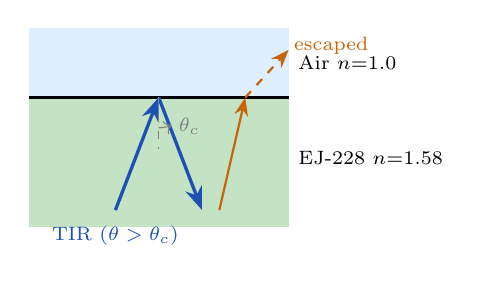
\begin{tikzpicture}[scale=1.1,every node/.style={font=\scriptsize}]
    % Interface
    \fill[airgap!60] (0,-0.05) rectangle (3.0,0.8);
    \fill[scintgr!30] (0,-1.5) rectangle (3.0,0.0);
    \draw[thick] (0,0) -- (3.0,0);
    \node[right] at (3.0,-0.7) {EJ-228 $n{=}1.58$};
    \node[right] at (3.0, 0.4) {Air $n{=}1.0$};

    % TIR ray
    \draw[vikuiti,very thick,-{Stealth}] (1.0,-1.3) -- (1.5,0);
    \draw[vikuiti,very thick,-{Stealth}] (1.5,0) -- (2.0,-1.3);
    \node[vikuiti] at (1.0,-1.6) {TIR ($\theta>\theta_c$)};

    % Escaping ray
    \draw[tironly,thick,-{Stealth}] (2.2,-1.3) -- (2.5,0);
    \draw[tironly,thick,-{Stealth},dashed] (2.5,0) -- (3.0,0.55);
    \node[tironly,right] at (2.95,0.6) {escaped};

    % Critical angle annotation
    \draw[gray,dashed] (1.5,0) -- (1.5,-0.6);
    \draw[gray,->] (1.5,-0.35) arc(270:295:0.35)
      node[right,pos=0.8] {$\theta_c$};
  \end{tikzpicture}
  \end{block}

  {\footnotesize
  The Vikuiti layer intercepts photons that escape TIR,
  reflecting them back into the scintillator with $R=0.98$.
  }
  \end{column}

\end{columns}

\end{frame}

% ─────────────────────────────────────────────────────────────────────────────
\section{Summary}

\begin{frame}{Summary \& Conclusions}

\begin{itemize}\setlength\itemsep{0.5em}

  \item[\textbf{1.}]
    An EJ-228 plastic scintillator cylinder ($\varnothing25\times\SI{25}{mm}$)
    was simulated with Geant4 11.4 MT in two reflector configurations:
    \textbf{Vikuiti 3M ESR} ($R=0.98$, specular) and \textbf{TIR-only}.

  \item[\textbf{2.}]
    Both caps are instrumented with $2\times2$ arrays of
    \SI{6x6}{mm^2} SiPMs (AFBR-S4N66P024M), 8 total.
    Horizontal 1\,GeV muons enter through the mantle.

  \item[\textbf{3.}]
    \textbf{Vikuiti increases light collection by $2.34\times$}
    ($\langle N_\text{pe}\rangle = 9663$ vs $4129$ per event).

  \item[\textbf{4.}]
    Detection efficiency: \textbf{20.3\% with Vikuiti} vs \textbf{8.7\% TIR-only}.
    The factor agrees with the simple analytical estimate
    ($f_\text{TIR} \approx 80\%$ trapped, $20\%$ recovered by Vikuiti).

  \item[\textbf{5.}]
    Top/bottom symmetry is excellent: $\langle N_\text{pe}\rangle_\text{top}
    \approx \langle N_\text{pe}\rangle_\text{bot}$ to $<0.05\%$, confirming
    Z-symmetric photon transport.

  \item[\textbf{6.}]
    A small SiPM-position asymmetry ($\sim 2\%$) is observed between
    $x=\pm\SI{3}{mm}$ SiPMs, consistent with the muon entry geometry.

\end{itemize}

\end{frame}

% ─────────────────────────────────────────────────────────────────────────────
\begin{frame}[plain]
  \begin{center}
    \Large\textbf{Appendix: Simulation Parameters}
  \end{center}

  \renewcommand{\arraystretch}{1.2}
  \begin{tabular}{@{}lll@{}}
    \toprule
    Parameter & Value & Notes \\
    \midrule
    Geant4 version   & 11.4.0 (MT) & 24 threads \\
    Events           & 5000 per config & Identical seed \\
    Physics list     & FTFP\_BERT + optical & Standard \\
    Optical model    & Unified (G4) & \\
    GROUPVEL fix     & $v_g = c/1.58$ in air & Prevents aliasing bug \\
    Scintillation    & Finite rise time & \SI{0.5}{ns} \\
    TIR $\theta_c$   & $39.3^\circ$ & $\arcsin(1/n)$ \\
    SiPM model       & PDE included & Wavelength-dependent \\
    Air gap thickness & \SI{0.1}{mm} & Mantle only \\
    Vikuiti thickness & \SI{0.1}{mm} & Structural = Mylar \\
    \bottomrule
  \end{tabular}

\vspace{1em}
{\footnotesize
Repository: \texttt{github.com/dowiyogo/ej200} \\
Branches: \texttt{feat/ej228-cylinder} (Vikuiti) |
          \texttt{feat/ej228-tir-only} (TIR-only)
}

\end{frame}

\end{document}
